\begin{appendices}

\section{\acf{he} Multiplication}
\label{app:he-multiplication}

In this section, we proof how the multiplication is achieved homomorphically between two encrypted vectors $[[x'_1]], [[x'_2]]$, as described in \cite{liu2016efficient2}.
It is worth mentioning that $[[x'_i]] = [[x_i]]^{r_{x_i}} = [[x_i . r_{x_i}]]$.
This step is performed for masking the value $x_i$ by adding a random value $r_{x_i}$ to it.
The formal definition of this function is $HE.Mul([[x'_1]], [[x'_2]]) \rightarrow [[x_{mul}]]$.
\Cref{fig:he-mul-explain} shows the operations for performing the multiplication operation between two parties $S_1, S_2$, where they hold the homomorphic secret key $sk_1, sk_2$, respectively.

\begin{figure*}[thb]
\centering
  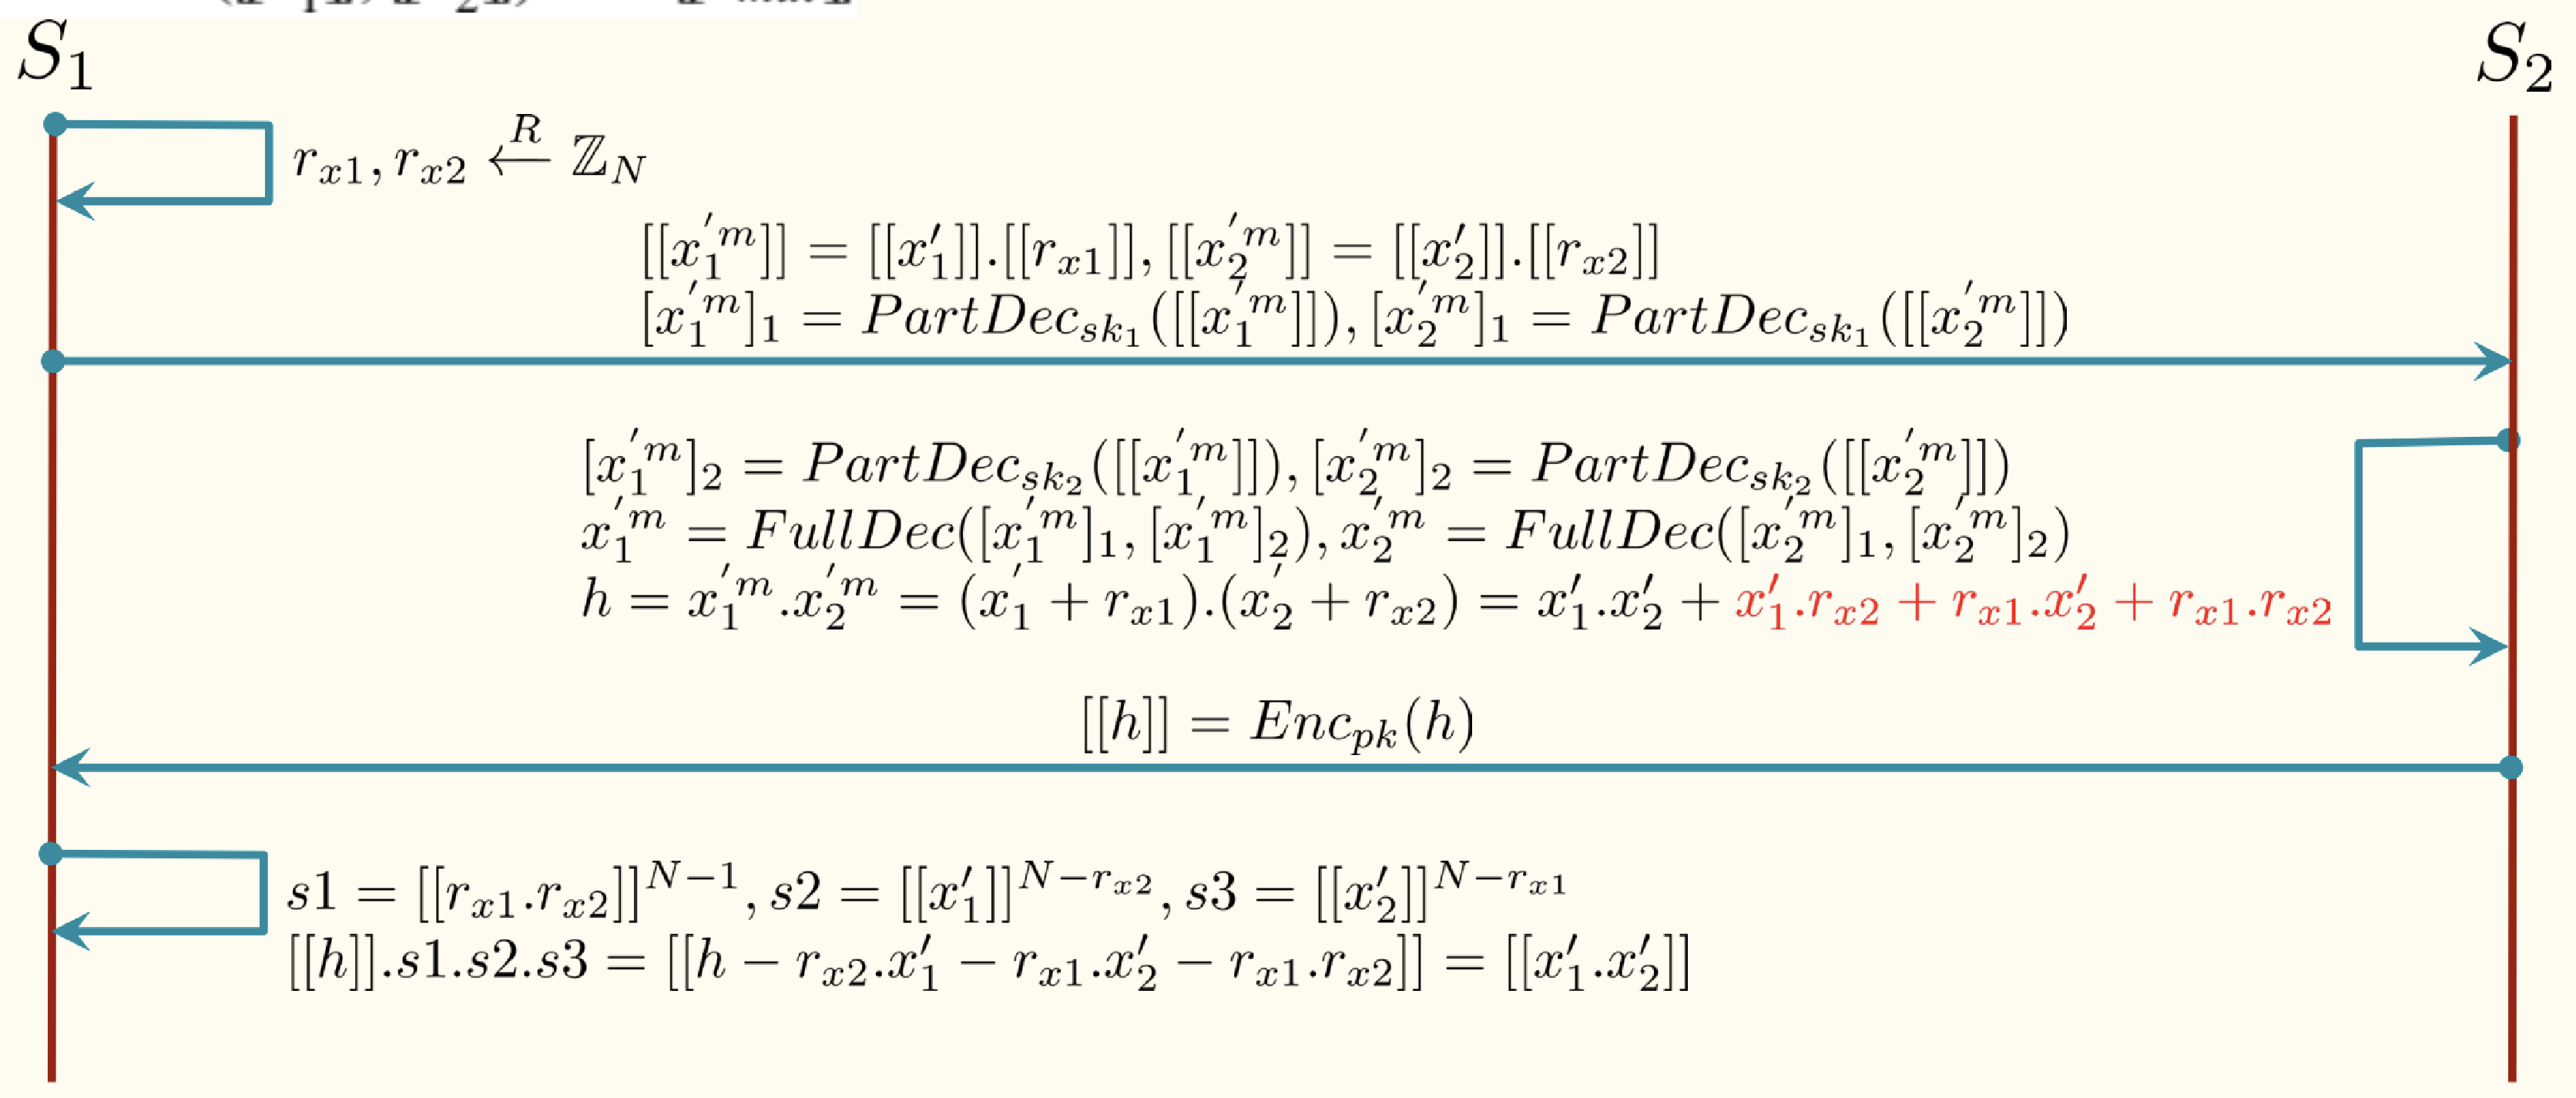
\includegraphics[width=1\linewidth]{resources/HE-mul-explain.pdf}
  \caption{HE multiplication explanation}
  \label{fig:he-mul-explain}
  %\vspace{-5mm}
\end{figure*}
    
% \section{Second Proof}
% \label{app:second-proof}

% This is the second appendix.
\end{appendices}
